
% \title{Apunte de Matemáticas Discretas CC3101:\\ Relaciones y funciones Clase 10}
% % \title{Ejercicios Lógica e Inducción}
% \author{Andrés Abeliuk}
% \date{}
% \maketitle


\section{Operaciones sobre Relaciones}

En esta secci\'on abordaremos c\'omo se pueden manipular las relaciones mediante operaciones, algunas heredadas de la teor\'ia de conjuntos y otras espec\'ificas de las relaciones. Esto permite construir relaciones m\'as complejas a partir de otras m\'as simples, analizar sus propiedades y establecer conexiones entre distintas estructuras.

\subsection{Operaciones Cl\'asicas: Uni\'on, Intersecci\'on y Diferencia}

Dado que una relaci\'on $R$ sobre un conjunto $A$ es un subconjunto de $A \times A$, podemos aplicar las operaciones usuales de conjuntos para combinarlas:

\begin{itemize}
  \item \textbf{Uni\'on:} $R \cup R'$ contiene todos los pares que pertenecen a $R$, a $R'$ o a ambos.
  \item \textbf{Intersecci\'on:} $R \cap R'$ contiene solo los pares comunes a ambas relaciones.
  \item \textbf{Diferencia:} $R \setminus R'$ contiene los pares que est\'an en $R$ pero no en $R'$.
\end{itemize}

Estas operaciones nos permiten combinar o contrastar relaciones distintas, como por ejemplo, intersectar relaciones de amistad y colaboraci\'on en redes sociales.


%
\subsection{Operaciones Espec\'ificas sobre Relaciones}

Adem\'as de las operaciones anteriores, existen operaciones espec\'ificas para relaciones:

\begin{itemize}
  \item \textbf{Inversi\'on:} La relaci\'on inversa de $R$ se denota $R^{-1}$ y consiste en invertir el orden de todos los pares: $R^{-1} = \{(b,a) \mid (a,b) \in R\}$.

  \item \textbf{Composici\'on:} Dadas dos relaciones $R \subseteq A \times B$ y $R' \subseteq B \times C$, su composici\'on es:
  \[ R' \circ R = \{(a,c) \mid \exists b. (a,b) \in R \land (b,c) \in R'\}. \]
  Esta operaci\'on se interpreta como ``relaci\'on indirecta'' a trav\'es de un intermediario.

  \item \textbf{Potencia:} Si $R$ es una relaci\'on sobre un conjunto $A$, definimos inductivamente:
  \[ R^1 = R, \quad R^{n+1} = R^n \circ R. \]
\end{itemize}

% Estas operaciones permiten, por ejemplo, analizar caminos de longitud $n$ en grafos (pensando en $R$ como relaci\'on de adyacencia).

\begin{figure}[H]
\centering
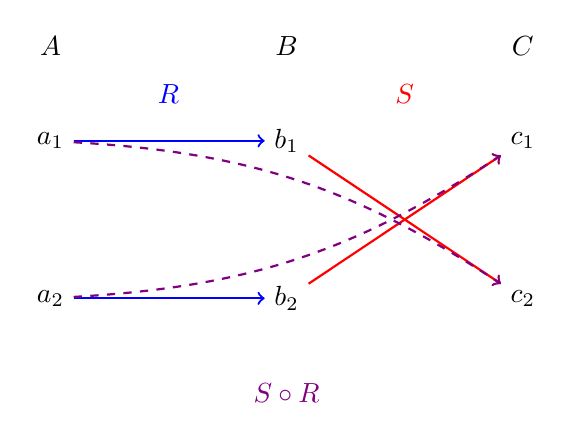
\begin{tikzpicture}[scale=1]

  % Conjuntos A, B, C
  \node (a1) at (0,2) {$a_1$};
  \node (a2) at (0,0) {$a_2$};

  \node (b1) at (3,2) {$b_1$};
  \node (b2) at (3,0) {$b_2$};

  \node (c1) at (6,2) {$c_1$};
  \node (c2) at (6,0) {$c_2$};

  % R: A -> B
  \draw[->, thick, blue] (a1) -- (b1);
  \draw[->, thick, blue] (a2) -- (b2);

  % S: B -> C
  \draw[->, thick, red] (b1) -- (c2);
  \draw[->, thick, red] (b2) -- (c1);

  % Composition: A -> C
  \draw[->, thick, dashed, violet] (a1) to[bend left=15] (c2);
  \draw[->, thick, dashed, violet] (a2) to[bend right=15] (c1);

  % Labels
  \node at (0,3.2) {$A$};
  \node at (3,3.2) {$B$};
  \node at (6,3.2) {$C$};

  % Legends
  \node[blue] at (1.5,2.6) {$R$};
  \node[red] at (4.5,2.6) {$S$};
  \node[violet] at (3, -1.2) {$S \circ R$};
\end{tikzpicture}
\caption{Composición de relaciones. Las flechas azules representan la relación \(R \subseteq A \times B\) y las rojas la relación \(S \subseteq B \times C\). La composición \(S \circ R \subseteq A \times C\) se indica con flechas punteadas moradas, que conectan elementos de \(A\) con \(C\) cuando existe un elemento intermedio en \(B\) que los vincula a través de \(R\) y \(S\).}
\end{figure}


\subsection*{Ejercicios resueltos}
\begin{exampleblock}{1. Transitividad y potencias:} Demostrar que $R$ es transitiva si y solo si $R^n \subseteq R$ para todo $n \geq 1$.

\emph{($\Rightarrow$)} Supongamos que $R$ es transitiva. Usamos inducción sobre $n$:

\textit{Caso base:} $n = 1$. Claramente $R^1 = R \subseteq R$.

\textit{Paso inductivo:} Supongamos que $R^k \subseteq R$. Entonces:
\[ R^{k+1} = R^k \circ R \subseteq R \circ R \subseteq R \]
por transitividad. Así, por inducción, $R^n \subseteq R$ para todo $n \geq 1$.

\emph{($\Leftarrow$)} Supongamos que $R^n \subseteq R$ para todo $n \geq 1$. En particular, $R^2 \subseteq R$ implica que $(a,b) \in R$ y $(b,c) \in R$ lleva a $(a,c) \in R^2 \subseteq R$, es decir, $R$ es transitiva.
\end{exampleblock}
\bigskip
\begin{exampleblock}{2. Simetría:} Demostrar que $R$ es simétrica si y solo si $R = R^{-1}$.

\emph{($\Rightarrow$)} Si $R$ es simétrica, entonces $(a,b) \in R$ implica $(b,a) \in R$, por lo tanto $R \subseteq R^{-1}$ y también $R^{-1} \subseteq R$, ya que si $(a,b) \in R^{-1}$ entonces $(b,a) \in R$ y por simetría $(a,b) \in R$. Así, $R = R^{-1}$.

\emph{($\Leftarrow$)} Si $R = R^{-1}$, entonces todo $(a,b) \in R$ satisface que $(b,a) \in R$, lo cual es precisamente la definición de simetría.
\end{exampleblock}
\bigskip
\begin{exampleblock}{3. Potencias de relación simétrica:} Sea $R$ simétrica. Demostrar que $R^n$ es simétrica para todo $n \geq 1$.

Demostramos por inducción sobre $n$ que $R^n$ es simétrica.

\textit{Caso base:} $n = 1$. $R^1 = R$ es simétrica por hipótesis.

\textit{Paso inductivo:} Supongamos que $R^k$ es simétrica. Consideremos $R^{k+1} = R^k \circ R$. Tomemos $(a,c) \in R^{k+1}$, entonces existe $b$ tal que $(a,b) \in R^k$ y $(b,c) \in R$. Por hipótesis, $(b,a) \in R^k$ y $(c,b) \in R$. Entonces $(c,a) \in R^{k+1}$, y se concluye que $R^{k+1}$ también es simétrica.

Así, $R^n$ es simétrica para todo $n \geq 1$.
\end{exampleblock}


\section{Clausuras}

Una clausura de una relaci\'on consiste en extenderla para que satisfaga una propiedad deseada (reflexividad, simetr\'ia o transitividad), agregando la menor cantidad posible de pares.

\begin{definitionblock}{Clausura}
Dada una relaci\'on $R$ sobre un conjunto $A$, su clausura reflexiva/sim\'etrica/transitiva es la \emph{menor} relaci\'on (en t\'erminos de inclusi\'on) que contiene a $R$ y que es reflexiva/sim\'etrica/transitiva, respectivamente.
\end{definitionblock}

\subsection{Clausura Reflexiva}

Se obtiene agregando todos los pares $(a,a)$ para cada $a \in A$ que no estaban ya en $R$.

\begin{exampleblock}{Ejemplo}
La clausura reflexiva de la relaci\'on $<$ sobre $\mathbb{N}$ es $\leq$.
\end{exampleblock}

\subsection{Clausura Sim\'etrica}

Para obtener la clausura sim\'etrica de una relaci\'on $R$, se agregan todos los pares $(b,a)$ tales que $(a,b) \in R$ pero $(b,a) \not\in R$.

\begin{exampleblock}{Ejemplo}
La clausura sim\'etrica de $R = \{(a,b) \mid a > b\}$ es $R \cup R^{-1} = \{(a,b) \mid a \neq b\}$.
\end{exampleblock}

\subsection{Clausura Transitiva}

La clausura transitiva de $R$ incluye todos los pares que se pueden alcanzar transitivamente:
\[ R^+ = \bigcup_{n=1}^{\infty} R^n. \]

La clausura reflexiva-transitiva se denota $R^* = R^+ \cup \{(a,a) \mid a \in A\}$.

\begin{exampleblock}{Ejemplo}
La clausura transitiva de la relaci\'on ``sucesor'' en $\mathbb{N}$ es la relaci\'on de orden $>$.
\end{exampleblock}


\begin{thmblock}{Lema}
Sea $R$ una relaci\'on sobre un conjunto finito $A$ con $|A| = n$. Demuestre que:
\[ R^+ = \bigcup_{1 \leq i \leq n} R^i. \]
\end{thmblock}
\begin{proof}
La clausura transitiva \( R^+ \) contiene todos los pares \((a,b)\) tales que existe un camino desde \( a \) hasta \( b \) siguiendo pasos de la relación \( R \).

En un conjunto finito con \( n \) elementos, cualquier secuencia de pasos que conecta dos elementos no necesita tener más de \( n \) pasos: si un camino tiene más de \( n \) nodos, entonces alguno se repite (por el principio del palomar que veremos en la próxima clase), y el camino puede acortarse eliminando ciclos.

Por lo tanto, para encontrar todos los pares conectados transitivamente, basta con considerar composiciones de \( R \) hasta longitud \( n \). 
\end{proof}

\begin{center}
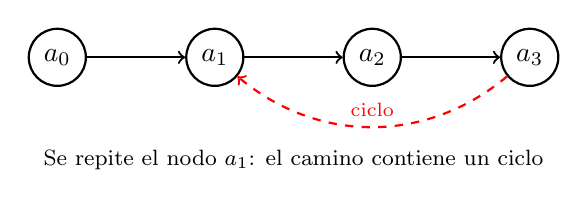
\begin{tikzpicture}[->, thick, node distance=2cm]
  % Nodos
  \node[circle,draw] (a0) at (0,0) {$a_0$};
  \node[circle,draw] (a1) at (2,0) {$a_1$};
  \node[circle,draw] (a2) at (4,0) {$a_2$};
  \node[circle,draw] (a3) at (6,0) {$a_3$};

  % Camino
  \draw[->] (a0) -- (a1);
  \draw[->] (a1) -- (a2);
  \draw[->] (a2) -- (a3);

  \draw[->, bend left=40, red, dashed] (a3) to node[above, sloped] {\scriptsize ciclo} (a1);

  % Nota
  \node at (3,-1.3) {\footnotesize Se repite el nodo $a_1$: el camino contiene un ciclo};
\end{tikzpicture}
\end{center}

\vspace{-0.5em}
\begin{center}
\textit{Figura:} Un camino de más de \( n \) pasos en un conjunto de \( n \) elementos debe repetir nodos. 
% El ciclo puede eliminarse, acortando el camino sin perder la conexión entre extremos.
\end{center}




\begin{exampleblock}{Ejemplo: Clausura transitiva en planificación de tareas}

Supongamos que tenemos un conjunto de tareas \( A = \{\text{A}, \text{B}, \text{C}, \text{D}\} \) en un proyecto. La relación \( R \subseteq A \times A \) indica dependencias directas: si \( (x, y) \in R \), entonces la tarea \( x \) debe completarse antes de comenzar la tarea \( y \).

Sean las dependencias directas:
\[
R = \{ (\text{A}, \text{B}), (\text{B}, \text{C}), (\text{C}, \text{D}) \}
\]

\textbf{Objetivo:} Calcular la clausura transitiva \( R^+ \), que representa todas las tareas que deben realizarse antes de otra, directa o indirectamente.

\textbf{Cálculo de \( R^+ \):}
\[
\begin{aligned}
R^1 &= R = \{ (\text{A}, \text{B}), (\text{B}, \text{C}), (\text{C}, \text{D}) \} \\\\
R^2 &= \{ (\text{A}, \text{C}), (\text{B}, \text{D}) \} \\\\
R^3 &= \{ (\text{A}, \text{D}) \} \\\\
R^+ &= R \cup R^2 \cup R^3 = \{ (\text{A}, \text{B}), (\text{B}, \text{C}), (\text{C}, \text{D}), (\text{A}, \text{C}), (\text{B}, \text{D}), (\text{A}, \text{D}) \}
\end{aligned}
\]

\textbf{Representación gráfica:}

\begin{center}
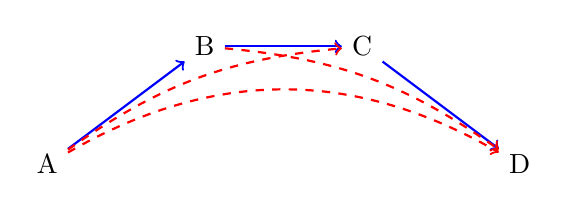
\begin{tikzpicture}[->, node distance=2cm, thick]
  \node (A) at (0, 0) {A};
  \node (B) at (2, 1.5) {B};
  \node (C) at (4, 1.5) {C};
  \node (D) at (6, 0) {D};

  % relaciones directas (R)
  \draw[->, blue] (A) -- (B);
  \draw[->, blue] (B) -- (C);
  \draw[->, blue] (C) -- (D);

  % relaciones transitivas (R+ \ R)
  \draw[->, dashed, red] (A) to[bend left=15] (C);
  \draw[->, dashed, red] (B) to[bend left=15] (D);
  \draw[->, dashed, red] (A) to[bend left=30] (D);
\end{tikzpicture}
\end{center}

\vspace{1mm}
{\small
\textcolor{blue}{Azul}: dependencias directas. \quad
\textcolor{red}{Rojo punteado}: dependencias inferidas transitivamente.
}

\end{exampleblock}


\section{Funciones}

\begin{definitionblock}{Funci\'on}
Una funci\'on $f: A \to B$ es una relaci\'on que a cada elemento $a \in A$ le asigna \emph{un \'unico} elemento $b \in B$. Se denota $f(a) = b$.
\end{definitionblock}

\noindent Dado $a \in A$ escribimos \textbf{$f(a)$} para denotar al \emph{único} $b \in B$ tal que $(a,b) \in f$. En este caso decimos que $b$ es la \textbf{imagen} de $a$ (o que $a$ es una \textbf{preimagen} de $b$).


\noindent El conjunto $A$ se llama \emph{dominio} y el conjunto $\{b \in B \mid \exists a \in A, f(a) = b\}$ se llama \emph{rango}.

\subsection{Clasificaci\'on de funciones}

\begin{itemize}
  \item \textbf{Inyectiva (uno a uno):} Si $a_1 \neq a_2$ implica $f(a_1) \neq f(a_2)$.
  \item \textbf{Sobreyectiva (sobre):} Si todo $b \in B$ tiene una preimagen en $A$.
  \item \textbf{Biyectiva:} Si es inyectiva y sobreyectiva.
\end{itemize}

\begin{exampleblock}{Ejemplos}
La funci\'on $f:\mathbb{N}_0 \to \mathbb{N}_0$ dada por $f(n) = 2n$ es inyectiva pero no sobreyectiva.

La funci\'on $f:\mathbb{N}_0 \to \mathbb{N}_0$ dada por $f(0) = 1$, $f(n) = n-1$ para $n>0$, es sobreyectiva pero no inyectiva.
\end{exampleblock}

\subsection{Operaciones con funciones}

\begin{itemize}
  \item \textbf{Composici\'on:} Dados $f: A \to B$ y $g: B \to C$, se define $g \circ f: A \to C$ por $g(f(a))$.
  \item \textbf{Inversa:} Si $f$ es biyectiva, entonces existe $f^{-1}: B \to A$ tal que $f^{-1}(f(a)) = a$.
\end{itemize}

\begin{exampleblock}{Ejercicio Propuesto}
Demuestre que si $f$ y $g$ son inyectivas (resp. sobreyectivas), entonces $g \circ f$ tambi\'en lo es.
\end{exampleblock}

\section{Crecimiento de Funciones}

Para comparar el comportamiento asint\'otico de funciones, usamos la notaci\'on $O$:

\begin{definitionblock}{Notaci\'on $O$}
Dadas funciones $f$ y $g$, decimos que $f(x)$ es $O(g(x))$ si existen constantes $c, k > 0$ tales que:
\[ f(x) \leq c \cdot g(x), \quad \forall x > k. \]
\end{definitionblock}

\begin{exampleblock}{Ejercicios Propuestos}
\begin{itemize}
\item Demuestre que $f(x) = x^2 + 2x + 1$ es $O(x^2)$.
\item Demuestre que todo polinomio de grado $n$ con coeficientes reales es $O(x^n)$.
\end{itemize}
\end{exampleblock}

\subsection{Composici\'on de funciones en t\'erminos de $O$}

\begin{thmblock}{Teorema}
Si $f_1 = O(g_1(x))$ y $f_2 = O(g_2(x))$, entonces:
\begin{itemize}
  \item $f_1(x) + f_2(x) = O(\max\{g_1(x), g_2(x)\})$.
  \item $f_1(x) \cdot f_2(x) = O(g_1(x) \cdot g_2(x))$.
\end{itemize}
\end{thmblock}
\begin{proof}
Por hipótesis, existen constantes positivas $c_1$, $k_1$ tales que
\[
f_1(x) \leq c_1 \cdot g_1(x), \quad \forall x > k_1,
\]
y constantes $c_2$, $k_2$ tales que
\[
f_2(x) \leq c_2 \cdot g_2(x), \quad \forall x > k_2.
\]

Sea $k = \max\{k_1, k_2\}$. Entonces para todo $x > k$, ambas desigualdades se cumplen.

\textbf{1. Suma:}
\[
f_1(x) + f_2(x) \leq c_1 g_1(x) + c_2 g_2(x) \leq (c_1 + c_2) \cdot \max\{g_1(x), g_2(x)\}.
\]
Por lo tanto, $f_1(x) + f_2(x) = O(\max\{g_1(x), g_2(x)\})$.

\textbf{2. Producto:}
\[
f_1(x) \cdot f_2(x) \leq (c_1 g_1(x)) \cdot (c_2 g_2(x)) = (c_1 c_2) \cdot g_1(x) g_2(x).
\]
Por lo tanto, $f_1(x) \cdot f_2(x) = O(g_1(x) \cdot g_2(x))$.
\end{proof}

\begin{exampleblock}{Ejercicios Propuestos}
\begin{itemize}
% \item Demuestre el teorema anterior.
\item Demuestre que $(x + 1)\log(x^2 + 1) + 3x^2$ es $O(x^2)$.
\end{itemize}
\end{exampleblock}